\section{Validation}

CLAS12 Trigger System Validation was initially performed on data samples simulated by GEANT when system was in design stage. When system was installed cosmic data were used. Finally when beam operation started, validation was complete as part of entire CLAS12 detector commissioning. Details discussed below.

\subsection{Validation during design phase}

Validation process consists of several methods and depends on the nature of validated trigger component. For stage1 components written on C++ for HLS/VIVADO implementation,
GEANT-simulated data were processed directly by C++ code and compared with initial similation parameters. 
In addition, the same samples were processed by offline reconstruction software and results compared with the trigger output. 
That double check method practicaly guarantees bug-free implementation. It was no single case when c++ implementation passed validation on
simulated data and failed on final validation stage. Most complicated stage1 components were validated using this method.

Some stage1, as well as all stage2 and stage3 components were implemented using VHDL. For those, VIVADO tools were used for validation diring design phase, in particular ...

\subsection{Validation of special purpose FPGA triggers using cosmic runs} 

Efficiency and spatial uniformity of cluster finding trigger described in Section 5.3 requires already calibrated calorimeters with pre-determined PMT gain and light attenuation constants loaded into the VTP/FPGA trigger firmware.  Calibration runs using a special purpose MIP trigger were used to obtain these constants.  This so-called "pixel trigger" used a simple multiplicity condition on 1D cluster size for each U,V,W view to reject undesirable muon trajectories and select normally incident tracks.  This reduced the trigger and data rate by 95$\%$ and ensured the same MIP energy was deposited for all possible triple intersections of single strips.  

The pixel trigger pipeline executes these steps in parallel, with user configurable parameters in bold:
  1) If FADC hit energy $>$ \textbf{EMIN}, make a pulse \textbf{HITWIDTH}*4ns for that strip.
  2) Look for coincidence of U,V,W pixel strip candidates from step 1.
  3) Evaluate multiplicity \textbf{EVALDELAY}*4ns clock cycles after the leading edge of a candidate pixel from step 2.
  4) Generate pixel trigger if multiplicity requirement is met and we still have a hit on U,V,and W. 

Additional configurable trigger elements were introduced, including a total energy sum threshold \textbf{ESUM} and a lookup table for triplets of strips which satisfy the geometrical constraint $dU+dV+dW=\textbf{DALITZ}$, where $d$ is the normalized distance to the hit strip indicated by the arrows in Fig. 6 and $\textbf{DALITZ}=2$ for perfect pixels.  The latter test was sometimes necessary to prevent noisy PMTs from saturating the multiplicity (N=3) trigger condition.  Offline analysis showed that about $90\%$ of pixel triggers satisfied the Dalitz test (Fig. 7), while adjacent calorimeter elements which did not use the trigger had a much smaller pixel fraction.  This suggests the pixel trigger helps to suppress events which undergo multiple scattering, which would trigger adjacent strips and violate the multiplicity requirement.
%%%%%%%%%%%%%%%%%%%%%%%%%%%%%%%%%%%%%%%%% F I G U R E %%%%%%%%%%%%%%%%%%%%%%%%%%%%%%%%%%%%%%%%%%
\begin{figure}[!htb]
 \centering
  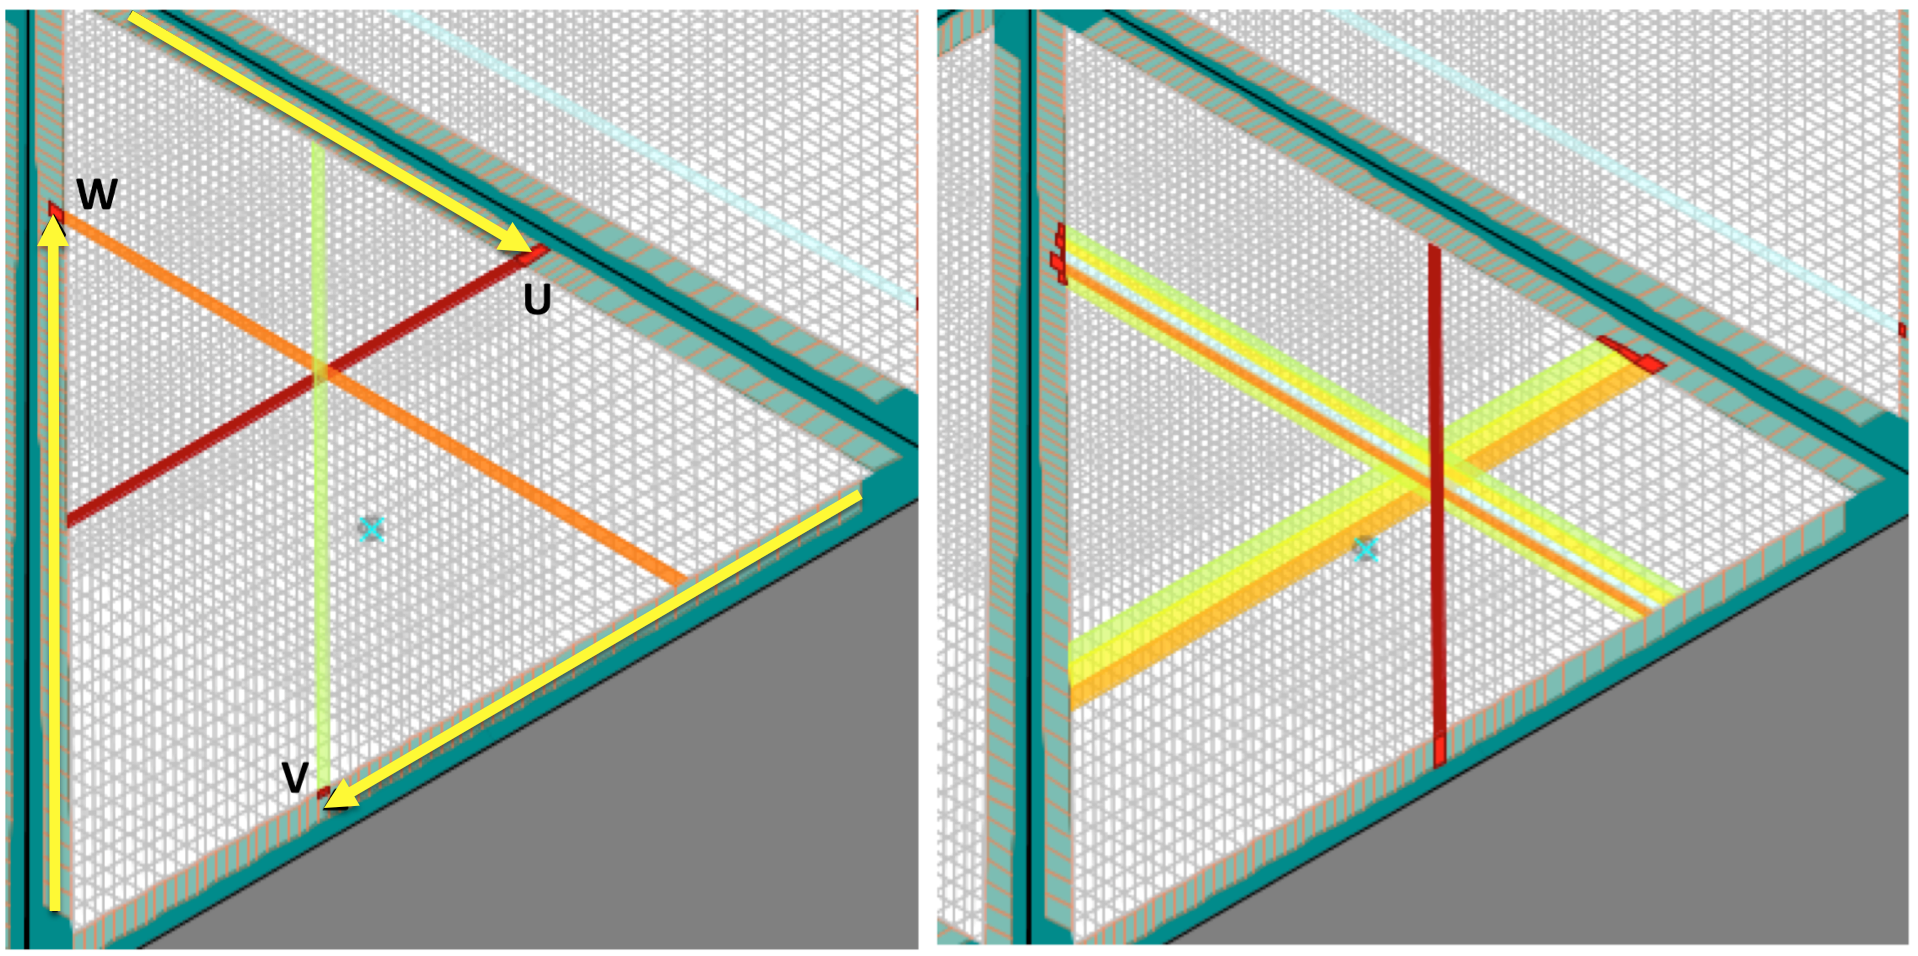
\includegraphics[width=0.95\columnwidth,keepaspectratio]{img/TwoClusters.png}
 \caption{Examples of clusters from cosmic muon triggers.  Desired trajectory (left) is normally incident on the face of PCAL and satisfies the single pixel multiplicity condition (N$_u$=N$_v$=N$_w$=1) in the FPGA pixel trigger.  Event at right shows a more vertical trajectory rejected by this trigger.}
\end{figure}
%%%%%%%%%%%%%%%%%%%%%%%%%%%%%%%%%%%%%%%%% F I G U R E %%%%%%%%%%%%%%%%%%%%%%%%%%%%%%%%%%%%%%%%%%

%%%%%%%%%%%%%%%%%%%%%%%%%%%%%%%%%%%%%%%%% F I G U R E %%%%%%%%%%%%%%%%%%%%%%%%%%%%%%%%%%%%%%%%%%
\begin{figure}[!htb]
 \centering
  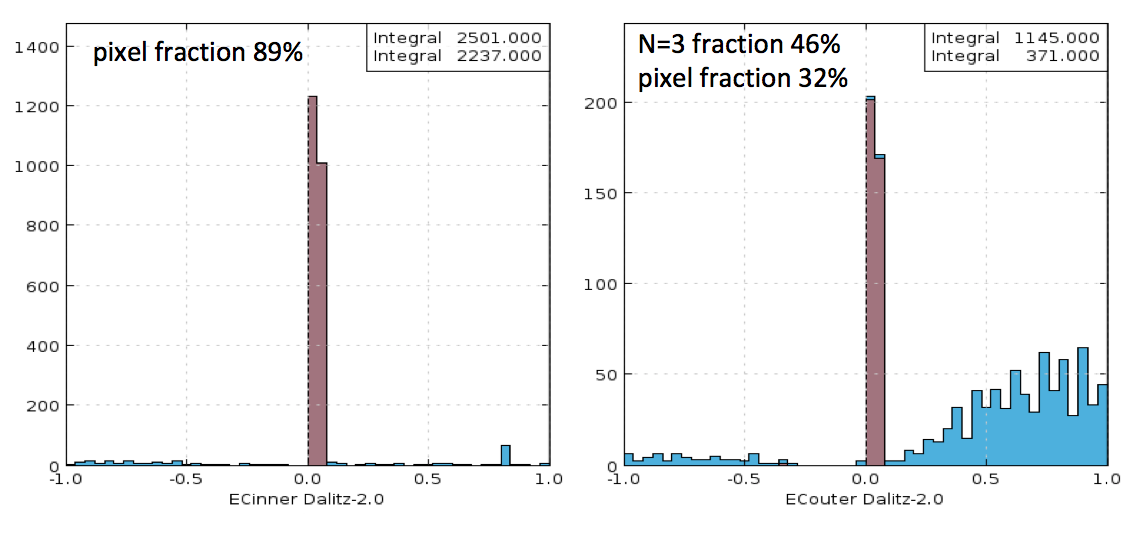
\includegraphics[width=1.0\columnwidth,keepaspectratio]{img/PixelFraction.png}
 \caption{Offline analysis of events which satisfied the pixel trigger on ECINNER calorimeter.  Left plot shows 89$\%$ of ECINNER triggers satisfied the pixel test $dU+dV+dW=2$.  Right plot shows only 14$\%$ of the ECINNER triggers found an ECOUTER event that satisfied both the $N=3$ and pixel test. }
\end{figure}
%%%%%%%%%%%%%%%%%%%%%%%%%%%%%%%%%%%%%%%%% F I G U R E %%%%%%%%%%%%%%%%%%%%%%%%%%%%%%%%%%%%%%%%%%
%\section{Validation on beam during CLAS12 detector commissioning - no FT} Rafo\\

\section{Validation of stage1 triggers using simulations}
Almost all of stage one trigger components, before deploying to the production firmware, were tested on GEANT4 simulated data.

\section{Validation of electron trigger based on ``Beam ON" data}
The ultimate validation of the trigger is done using the so called ''Random Trigger" (RT) runs.
RT runs are special runs, where event readout is initiated not by the trigger logic, but by an external random generator, that
can be tuned on the desired frequency. Most of events in RT runs will not contain any tracks, or other useful information, however,
small fraction of events will have real reconstructed particles which were reconstructed because accidentally detector's response
signal to the particle felled in the readout window that was initiated by the random generator.
Int the event readout in addition to various detector signals, the trigger decisions are stored as well (see section {\color{Red} XX, somewhere above
it should be described, how trigger decisions are made, and what is the clock cycle for trig decisions }).

We want to use these accidental ``Good" events, and check whether corresponding trigger bit is set by trigger logic ({\color{Red} I assume
trigger bits will be described above}).
%%%%%%%%%%%%%%%%%%%%%%%%%%%%%%%%%%%%%%%%% F I G U R E %%%%%%%%%%%%%%%%%%%%%%%%%%%%%%%%%%%%%%%%%%
\begin{figure}[!htb]
 \centering
 \subfloat[]{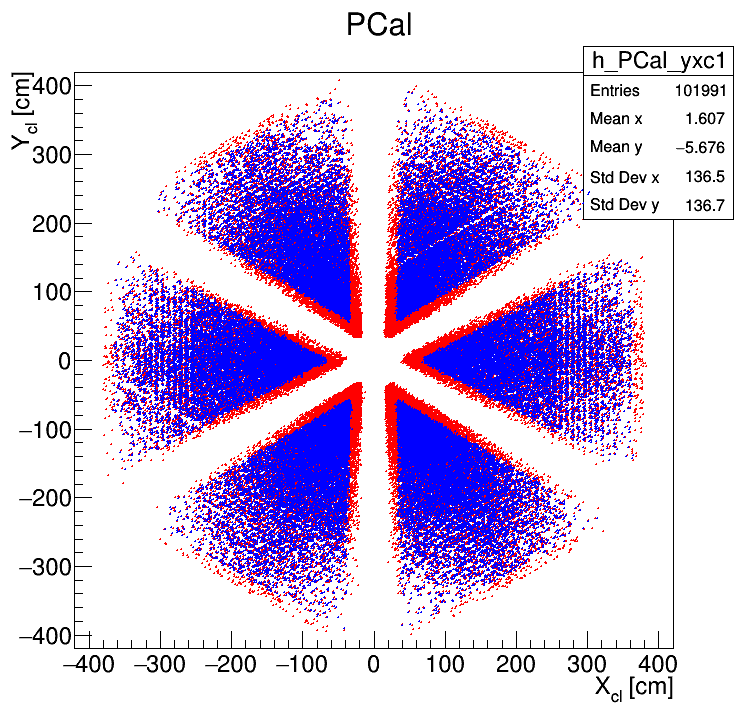
\includegraphics[width=0.24\textwidth]{img/PCal_Fiducials_4878.png}}
 \subfloat[]{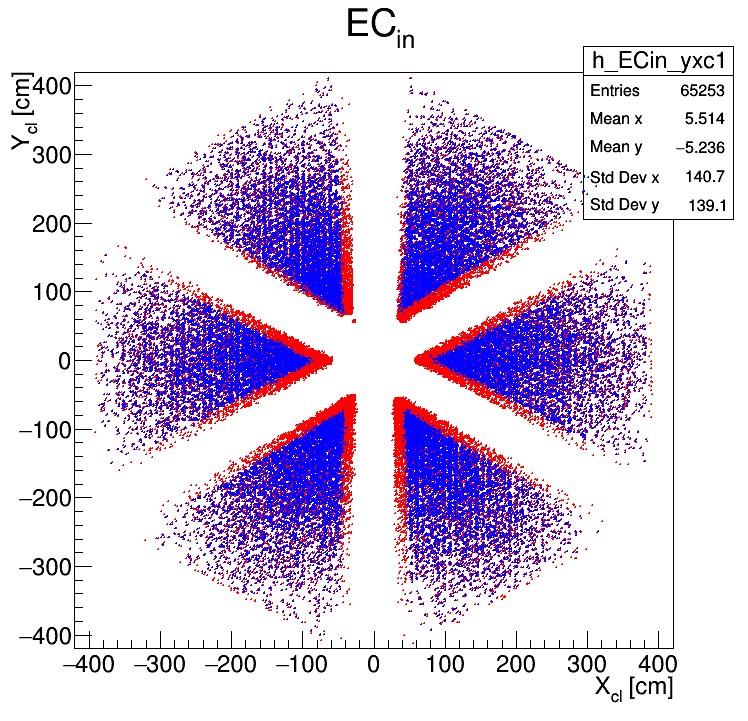
\includegraphics[width=0.24\textwidth]{img/ECin_Fiducials_4878.png}}
 \caption{Distribution of cluster coordinates of PCal (left) and EC\_{in} (right).
 scatter plot in Red shows all events, while blue scatter plot show events where cluster
 is in the fiducial region of the calorimeter (about 15 cm away from the edges).}
\end{figure}
%%%%%%%%%%%%%%%%%%%%%%%%%%%%%%%%%%%%%%%%% F I G U R E %%%%%%%%%%%%%%%%%%%%%%%%%%%%%%%%%%%%%%%%%%

The technique of the trigger validation is the following,
Analysing RT runs, we select 

\subsection{Validation on beam during CLAS12 detector commissioning -  photoproduction trigger}

As described in section \ref{sec:photoproduction_trigger}, the CLAS12 photoproduction trigger requires the coincidence between one electron measured in the Forward Tagger detector, and two hadrons measured within the CLAS12 detector, in the forward or central part. The validation procedure aims to verify if, for a given event foreseeing one final-state electron in the FT acceptance and two or more hadrons scattered within the CLAS12 acceptance, the trigger system would recognize it properly, resulting in event readout. In order to validate the system with beam during commissioning, the following strategy was adopted. First, the $e^-$ detection by the FT was validated using Random Trigger runs. After this, the detection of single hadrons in CLAS12 was studied in special runs, were the only trigger source was the FT. Finally, the coincidence between the two systems was assessed.

\subsubsection{Validation of $e^-$ detection in FT}

A scattered electron in the Forward Tagger is identified as an electromagnetic shower in the Forward Tagger Calorimeter within a proper energy range, in time coincidence and geometrically matched to a hit in both layers of the Forward Tagger Hodoscope. The map providing the matching between the cluster seed position in the FT-Cal and the tiles position in the FT-Hodo was first derived by the nominal detector geometry, and then confirmed by Montecarlo simulations.

The identification of the scattered $e^-$ in the FT was validated through a similar procedure as the one adopted for the CLAS12 electron trigger discussed before, based on ``Random Trigger'' runs. Recorded events were processed through the standard CLAS12 reconstruction software and filtered, keeping only those with a reconstructed $e^-$ in the FT system. Since event readout was triggered by a random pulser, events with the reconstructed $e^-$ signal close to the margins of the readout window were also rejected.
For these events, the electromagnetic clusters found by the reconstruction software (``offline'' clusters) were compared to those reported by the trigger system and stored in the form of the trigger data banks.

The efficiency of the FT-Cal clustering algorithm in the trigger system was evaluated by comparing all ``offline'' clusters to those matched - in space and time - to an ``online'' one\footnote{The energy of ``offline'' clusters is properly corrected to account for electromagnetic shower leakage from the bak of the FT-Cal, while ``online'' clusters do not implement this. Therefore, for a given $e^-$ in the FT-Cal, there is a systematic difference between the two energies. This effect is properly taken into account when setting the energy range for $e^-$ detection in the trigger system, and does not affect the corresponding trigger efficiency.}. The efficiency was computed as:
\begin{equation}
\varepsilon=\frac{N_{trigger}}{N_{all}} \; ,
\end{equation}
where $N_{all}$ and $N_{trigger}$ are, respectively, the total number of ``offline'' clusters and the number of ``offline'' clusters matched to an ``online'' one.
The result is shown in Fig.~\ref{fig:FT_ClusterEfficiency}, reporting the FT trigger efficiency for electromagnetic clusters as a function of the corresponding corrected energy. Efficiency is higher than 97.5$\%$ in the full energy range of interest / 99.5$\%$ in the energy range above 1 GeV. The difference is mainly due to the fact that the clustering algorithm in the trigger system works on a 3x3 matrix of crystals, whereas this limitation doesn't hold in the offline reconstruction.
The efficiency of the FT-Cal / FT-Hodo matching algorithm was evaluated in a similar way, repeating previous calculation but considering only electromagnetic clusters associated to one hit in each FT-Hodo layer. The result is reported in Fig.~\ref{fig:FT_ClusterEfficiencyHODO}.

%%%%%%%%%%%%%%%%%%%%%%%%%%%%%%%%%%%%%%%%% F I G U R E %%%%%%%%%%%%%%%%%%%%%%%%%%%%%%%%%%%%%%%%%%
\begin{figure}[!htb]
 \centering
{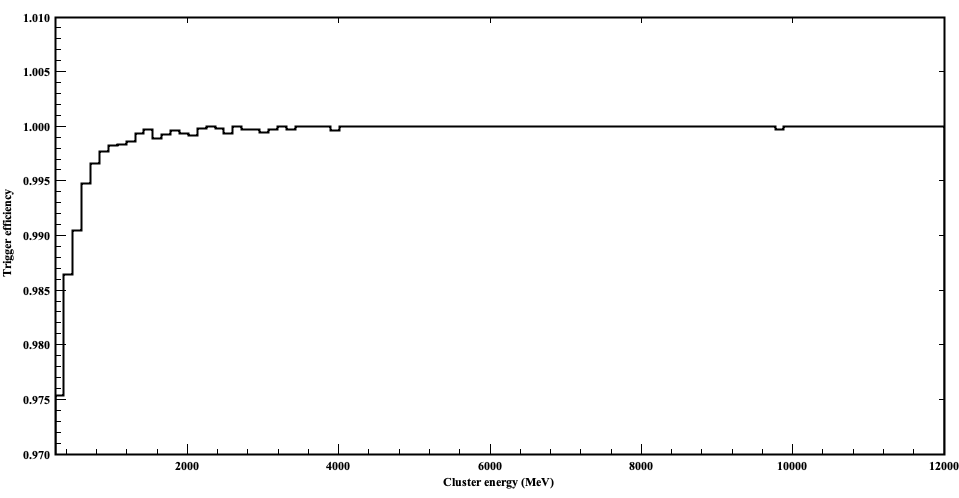
\includegraphics[width=.5\textwidth]{img/FT_ClusterEfficiency.png}}
 \caption{TODO: better figure, with errors (run 4288)}
 \label{fig:FT_ClusterEfficiency}
\end{figure}
%%%%%%%%%%%%%%%%%%%%%%%%%%%%%%%%%%%%%%%%% F I G U R E %%%%%%%%%%%%%%%%%%%%%%%%%%%%%%%%%%%%%%%%%%




\subsubsection{Validation of charged hadrons detection in CLAS12-FD}

The trigger system recognizes a charged hadron in the CLAS12 forward detector as a hit in the Forward Time-Of-Flight system (panel 1B) in time coincidence and geometrically matched to a hit in the U-bars of the Preshower Calorimeter, associated to a cluster with energy larger than a programmable threshold. The map providing the geometrical matching between FTOF counter and the PCAL U-bar was first derived by the nominal detector geometry, and then confirmed by Montecarlo simulations. To reduce the rate of random coincidences, the trigger system also requires the presence of a segment in 5 out of 6 drift chamber layers. The charged hadron identification algorithm was validated in special data-taking runs in which the Forward Tagger was the only enabled event readout source. In these runs, the trigger system was configured to report in the output trigger bank the presence of a charged hadron in any CLAS12-FD sector, as defined before. 

Recorded events were processed through standard reconstruction software and filtered, keeping only those with a well reconstructed charged track measured in CLAS12-FD. The track was required to be within the nominal acceptance of CLAS12 PCAL, and a momentum threshold of 300 MeV/c was applied. The trigger system efficiency was evaluated by comparing all reconstructed tracks to the tracks recognized by the trigger system. During commissioning, the efficiency was evaluated as a function of different observables, such as the energy deposited in the FTOF counters and in the PCAL, and the topology of the geometrical matching window. Trigger parameters were individually tuned to maximize the trigger efficiency. In the final configuration, an energy threshold of 2 MeV and 10 MeV for the FTOF counters and PCAL clusters was selected.  The result is reported in Fig.~\ref{fig:FD_TrackEfficiency}, showing the CLAS12-FD trigger efficiency for charged hadrons as a function of the track momentum. The efficiency is larger than 99$\%$ in the full momentum range, the inefficiency being dominated by threshold effects for the PCAL clusters.

%%%%%%%%%%%%%%%%%%%%%%%%%%%%%%%%%%%%%%%%% F I G U R E %%%%%%%%%%%%%%%%%%%%%%%%%%%%%%%%%%%%%%%%%%
\begin{figure}[!htb]
 \centering
{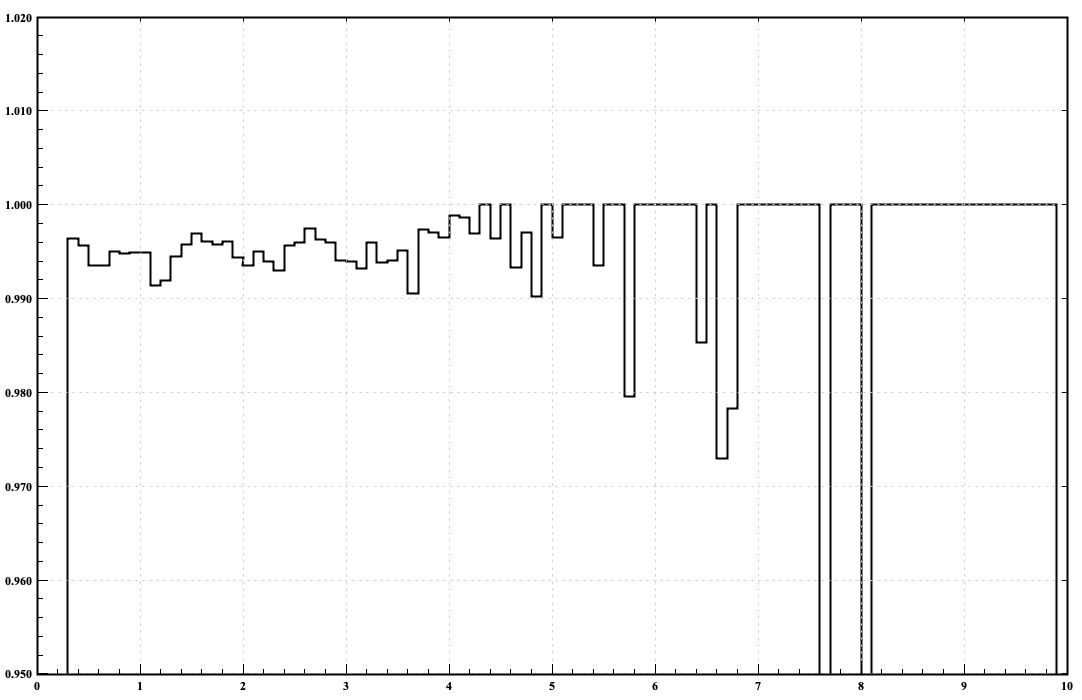
\includegraphics[width=.5\textwidth]{img/FD_TrackEfficiency.png}}
 \caption{TODO: better figure, with errors - run 5049-5050 (run4)}
 \label{fig:FD_TrackEfficiency}
\end{figure}
%%%%%%%%%%%%%%%%%%%%%%%%%%%%%%%%%%%%%%%%% F I G U R E %%%%%%%%%%%%%%%%%%%%%%%%%%%%%%%%%%%%%%%%%%



\subsubsection{Validation of charged hadron detection in CLAS12-CD}

The trigger system recognizes a charged hadron in the CLAS12 central detector as a hit in the Time-Of-Flight system (panel 1B) in time coincidence and geometrically matched to a hit in the U-bars of the Preshower Calorimeter.




\subsection{Final validation before experiment start up}

After CLAS12 detector was commissioned and trigger system components were validated, we still have to execute validation process for entire system in the begining of every experiment. It is needed because different experiments requesting configuration changes in trigger system, taking advantage of it's flexibility. Also, we are applying firmware changes occasionally to improve trigger system components based on previous experience, and those changes have to be validated.
Final trigger system validation is performed by taking beam data with random trigger (see ~\ref{sec:validation_random}).

Final trigger validation procedure was executed several times during first year of CLAS12 experiments and it was proven to be very useful: bugs in trigger firmware were found and fixed, and trigger configuration parameters were optimized.
For one occasion firmware bug was introduced into PCAL stage1 trigger logic during firmware update which expected to be small and simple. Final validation procedure revealed irregulatity in spacial distribution of clusters (fig ~\ref{fig:PCAL_bug_data}) (it also shows one CLAS12 sector is missing but it was enother problem unrelated to the trigger system). Since PCAL stage1 firmware is implemented in C++/HLS, GEANT4 data sample was reprocessed through C++ firmware implementation (fig. ~\ref{fig:PCAL_bug_hls}), problem was confirmed and subsequently found and fixed. Firmware was recompiled and reloaded and final trigger validation was repeated showing that problem was fixed. It took just several hours between finding the problem and being ready to run again. Every experiment in CLAS12 starts from final trigger system validation. 

\begin{figure}[hbt]
	\centering
	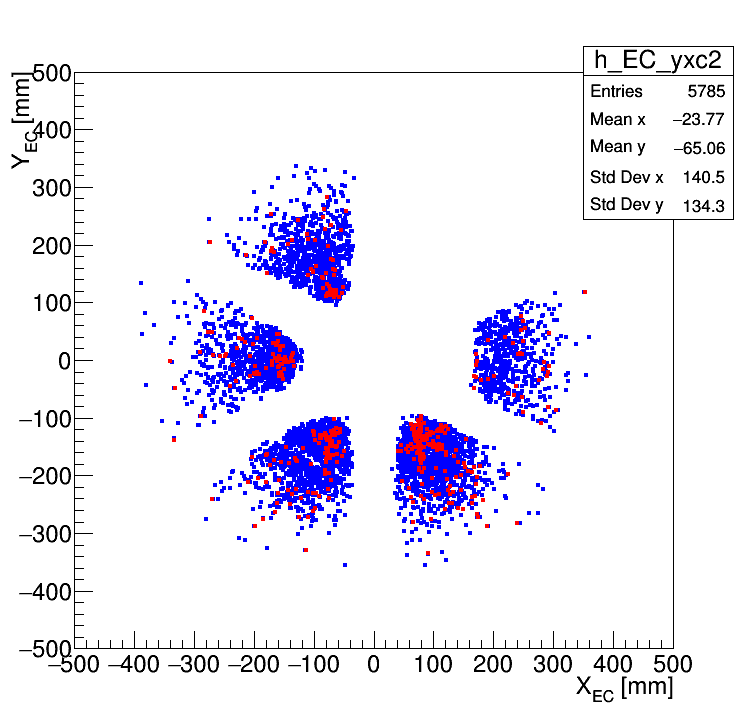
\includegraphics[width=1.0\columnwidth,keepaspectratio]{img/PCAL_bug_data.png}
	\caption{PCAL bug in beam data}
	\label{fig:PCAL_bug_data}
\end{figure}

\begin{figure}[hbt]
	\centering
	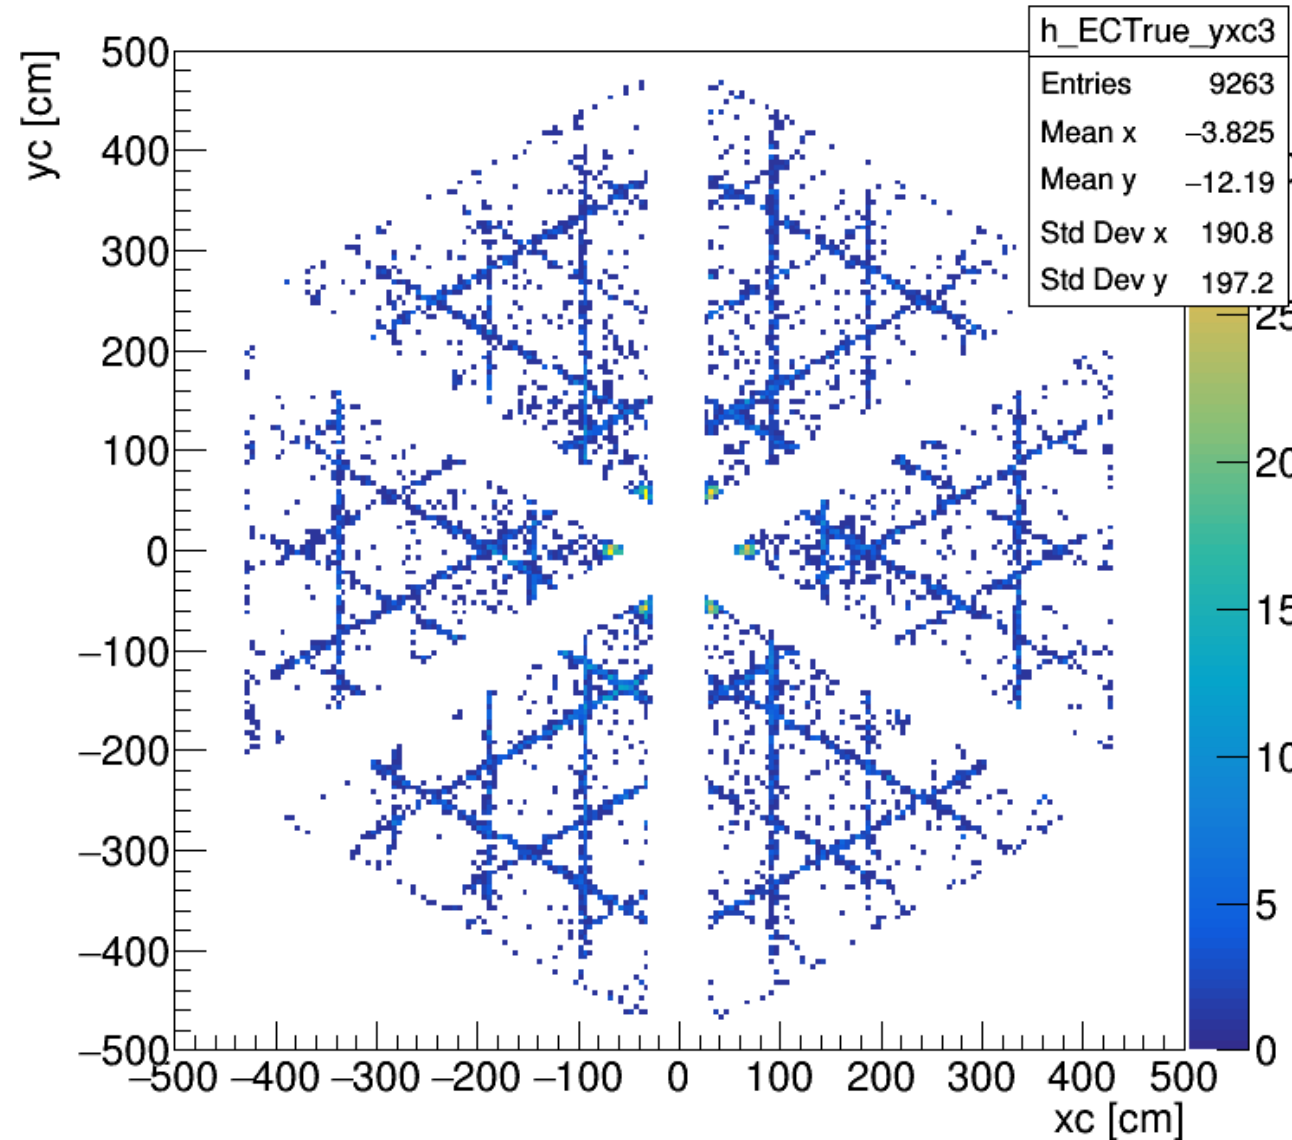
\includegraphics[width=1.0\columnwidth,keepaspectratio]{img/PCAL_bug_hls.png}
	\caption{PCAL bug in GEANT4 simulation}
	\label{fig:PCAL_bug_hls}
\end{figure}

